% Author: Dominik Harmim <harmim6@gmail.com>

\documentclass[a4paper, 11pt]{scrartcl}

\usepackage[czech]{babel}
\usepackage[utf8]{inputenc}
\usepackage[T1]{fontenc}
\usepackage{times}
\usepackage[left=2cm, top=3cm, text={17cm, 24cm}]{geometry}
\usepackage[unicode, colorlinks, hypertexnames=false, citecolor=red]{hyperref}
\usepackage{fancyhdr}
\usepackage{lastpage}
\usepackage{amssymb}
\usepackage{amsmath}
\usepackage{graphicx}

\newcommand{\TASK}{2: Časované automaty}
\newcommand{\COURSE}{Analýza systémů založená na modelech}
\newcommand{\AUTHOR}{Dominik Harmim (xharmi00)}

\newcommand*{\QEDB}{\hfill\ensuremath{\square}}

\pagestyle{fancy}
\fancyhead[L]{\AUTHOR}
\fancyhead[C]{\COURSE}
\fancyhead[R]{\today}

\fancyfoot[C]{}
\fancyfoot[R]{\thepage\,/\,\pageref*{LastPage}}

\setlength{\parindent}{0pt}


\begin{document}
    \begin{center}
        {\Large Úloha~\TASK}
    \end{center}


    \section*{1.~příklad}

    \begin{itemize}
        \item
            \textbf{Automat~$ \boldsymbol{\mathcal{A}_1} $ obsahuje \emph{zeno
            běh}.} Např. běh $ \rho = (A; x = 0, y = 0) \xrightarrow{\mathtt{
            a_1}} (B; x = 0, y = 0) \xrightarrow{\mathtt{a_2}} (C; x = 0, y = 0)
            \xrightarrow{\mathtt{a_4}} (A; x = 0, y = 0) \xrightarrow{\mathtt{
            a_1}} \dots $ je zeno běh, protože je to \emph{časově konvergentní
            nekonečný běh} ($ Exectime(\rho) = 0 $), který obsahuje \emph{
            nekonečné množství diskrétních kroků}. \textbf{Neplatí zde také
            \emph{podmínka neexistence zeno běhu}}, protože pro \emph{řídící
            cyklus} $ A \xrightarrow{g_1, \mathtt{a_1}, R_1} B \xrightarrow{g_2,
            \mathtt{a_2}, R_2} C \xrightarrow{g_4, \mathtt{a_4}, R_4} A $
            neexistují hodiny, pro které by alespoň jeden krok cyklu vyžadoval
            běh času. Jinými slovy, $ \nexists\,x \in \mathcal{C}: \exists\,i
            \in \{1, 2, 4\}: \exists\,c \in \mathbb{N}^+: \nu(x) < c
            \Rightarrow \nu(x) \not\models g_i $. \QEDB

        \item
            \textbf{Automat~$ \boldsymbol{\mathcal{A}_1} $ obsahuje
            \emph{timelock}.} \textbf{Běh vedoucí do timelocku je např.
            následující: \\
            $ \boldsymbol{(A; x = 0, y = 0) \xrightarrow{10} (A; x = 10, y =
            10)} $.} \emph{Konfigurace} $ c = (A; x = 10, y = 10) $ je
            timelock, protože $ Paths_{div}(c) = \emptyset $. Z~této
            konfigurace už není možné přejít do žádného jiného místa
            \emph{diskrétním krokem}, protože přechod do místa~B je podmíněn
            predikátem $ x \leq 1 $ a~přechod do místa~C je podmíněn predikátem
            $ 1 < x < 10 $. Tyto nejsou splněny, protože $ x = 10 $. Je zde
            pouze možné provádět \emph{nekonečné množství časových kroků},
            které ale vždy konvergují k~číslu~15, protože je v~místě~A
            \emph{invariant} $ y < 15 $. Žádný \emph{časově divergentní běh}
            tedy z~této konfigurace není možné provést. \QEDB
    \end{itemize}


    \section*{2.~příklad}

    Dále v~tomto příkladu budou uvažovány \emph{časované automaty} definovány
    následovně: \\
    $ \boldsymbol{\mathcal{A} = (Loc, Act, \mathcal{C}, \hookrightarrow,
    Loc_0, Inv, AP, L, Loc_{acc})} $, kde:
    \begin{itemize}
        \item
            $ Loc $ je konečná množina míst,

        \item
            $ Act $ je konečná množina událostí,

        \item
            $ \mathcal{C} $~je konečná množina hodin,

        \item
            $ \hookrightarrow\ \subseteq Loc \times CC(\mathcal{C}) \times
            Act \times 2^\mathcal{C} \times Loc $ je konečná množina přechodů,

            \begin{itemize}
                \item
                    $ CC(\mathcal{C}) = \{\bigwedge G\,|\,G \subseteq
                    ACC(\mathcal{C})\} $ je množina podmínek,

                \item
                    $ ACC(\mathcal{C}) = \{x \bowtie c\,|\,x \in \mathcal{C}
                    \wedge c \in \mathbb{N}\} $ je množina \emph{atomických
                    podmínek}, kde $ \bowtie\ \in \{<, \leq, =, \geq, >\} $,
            \end{itemize}

        \item
            $ Loc_0 \subseteq Loc $ je množina počátečních míst,

        \item
            $ Inv \subseteq Loc \times CC(\mathcal{C}) $ je konečná množina
            \emph{invariantů},

        \item
            $ AP $ je konečná množina \emph{atomických výroků},

        \item
            $ L \subseteq Loc \times 2^{AP} $ je ohodnocení míst,

        \item
            $ Loc_{acc} \subseteq Loc $ je množina koncových míst.
    \end{itemize}
    Dále jsou také uvažovány \emph{jazyky časovaných automatů}
    $ \boldsymbol{\mathcal{L}(\mathcal{A}) = \{w\,|\,w\ \text{\textbf{je
    přijato automatem}}~\mathcal{A}\}} $ nad \emph{konečnými slovy}
    $ \boldsymbol{w \in (Act \times \mathbb{R}^+)^*} $. \\

    \textbf{Důkaz uzavřenosti časovaných automatů vůči operaci
    \emph{sjednocení}:}
    \begin{itemize}
        \item
            Mějme dva jazyky časovaných automatů~$ L_{\mathcal{A}_1} $
            a~$ L_{\mathcal{A}_2} $. Dokažme, že jejich sjednocení
            $ L_{\mathcal{A}_1} \cup L_{\mathcal{A}_2} $ je opět jazyk
            časovaných automatů.

        \item
            Protože~$ L_{\mathcal{A}_1} $ a~$ L_{\mathcal{A}_2} $ jsou
            jazyky časovaných automatů, tak existují časované
            automaty~$ \mathcal{A}_1 $ a~$ \mathcal{A}_2 $, které přijímají
            jazyky~$ L_{\mathcal{A}_1} $ a~$ L_{\mathcal{A}_2} $, tj.
            $ L(\mathcal{A}_1) = L_{\mathcal{A}_1} $ a~$ L(\mathcal{A}_2) =
            L_{\mathcal{A}_2} $.

        \item
            Sestrojením časovaného automatu~$ \mathcal{A}_\cup $, který bude
            přijímat jazyk $ L_{\mathcal{A}_1} \cup L_{\mathcal{A}_2} $, tj.
            $ L(\mathcal{A}_\cup) = L(\mathcal{A}_1) \cup L(\mathcal{A}_2) $,
            dokážeme, že jazyk $ L_{\mathcal{A}_1} \cup L_{\mathcal{A}_2} $
            je jazyk časovaných automatů a~že operace sjednocení je uzavřena
            na časovaných automatech.
    \end{itemize}
    \vspace{-5pt}
    \textbf{Algoritmus sestrojení časovaného automatu~$ \boldsymbol{\mathcal{
    A}_\cup} $:}
    \begin{addmargin}[10pt]{0pt}
        \underline{Vstup:}
            Časovaný automat $ \mathcal{A}_1 = (Loc_1, Act_1, \mathcal{C}_1,
            \hookrightarrow_1, Loc_{0_1}, Inv_1, AP_1, L_1, Loc_{acc_1}) $
            a~časovaný automat $ \mathcal{A}_2 = (Loc_2, Act_2, \mathcal{C}_2,
            \hookrightarrow_2, Loc_{0_2}, Inv_2, AP_2, L_2, Loc_{acc_2}) $, kde
            bez újmy na obecnosti předpokládáme, že $ Loc_1 \cap Loc_2 =
            \emptyset $.
        \\[5pt]
        \underline{Výstup:}
            Časovaný automat $ \mathcal{A}_\cup = (Loc, Act, \mathcal{C},
            \hookrightarrow, Loc_0, Inv, AP, L, Loc_{acc}) $, kde
            $ L(\mathcal{A}_\cup) = L(\mathcal{A}_1) \cup L(\mathcal{A}_2) $.
        \\[5pt]
        \underline{Metoda:}
            \begin{enumerate}
                \item
                    $ Loc = Loc_1 \cup Loc_2 $.

                \item
                    $ Act = Act_1 \cup Act_2 $.

                \item
                    $ \mathcal{C} = \mathcal{C}_1 \cup \mathcal{C}_2 $.

                \item
                    $ \hookrightarrow\ =\ \hookrightarrow_1 \cup
                    \hookrightarrow_2 $.

                \item
                    $ Loc_0 = Loc_{0_1} \cup Loc_{0_2} $.

                \item
                    $ Inv = Inv_1 \cup Inv_2 $.

                \item
                    $ AP = AP_1 \cup AP_2 $.

                \item
                    $ L = L_1 \cup L_2 $.

                \item
                    $ Loc_{acc} = Loc_{acc_1} \cup Loc_{acc_2} $.
            \end{enumerate}
    \end{addmargin}
    \QEDB

    \textbf{Důkaz uzavřenosti časovaných automatů vůči operaci
    \emph{konkatenace}:}
    \begin{itemize}
        \item
            Mějme dva jazyky časovaných automatů~$ L_{\mathcal{A}_1} $
            a~$ L_{\mathcal{A}_2} $. Dokažme, že jejich konkatenace
            $ L_{\mathcal{A}_1} . L_{\mathcal{A}_2} $ je opět jazyk
            časovaných automatů.

        \item
            Protože~$ L_{\mathcal{A}_1} $ a~$ L_{\mathcal{A}_2} $ jsou
            jazyky časovaných automatů, tak existují časované
            automaty~$ \mathcal{A}_1 $ a~$ \mathcal{A}_2 $, které přijímají
            jazyky~$ L_{\mathcal{A}_1} $ a~$ L_{\mathcal{A}_2} $, tj.
            $ L(\mathcal{A}_1) = L_{\mathcal{A}_1} $ a~$ L(\mathcal{A}_2) =
            L_{\mathcal{A}_2} $.

        \item
            Sestrojením časovaného automatu~$ \mathcal{A}_\circ $, který bude
            přijímat jazyk $ L_{\mathcal{A}_1} . L_{\mathcal{A}_2} $, tj.
            $ L(\mathcal{A}_\circ) = L(\mathcal{A}_1) . L(\mathcal{A}_2) $,
            dokážeme, že jazyk $ L_{\mathcal{A}_1} . L_{\mathcal{A}_2} $
            je jazyk časovaných automatů a~že operace konkatenace je uzavřena
            na časovaných automatech.
    \end{itemize}
    \vspace{-5pt}
    \textbf{Algoritmus sestrojení časovaného automatu~$ \boldsymbol{\mathcal{
    A}_\circ} $:}
    \begin{addmargin}[10pt]{0pt}
        \underline{Vstup:}
            Časovaný automat $ \mathcal{A}_1 = (Loc_1, Act_1, \mathcal{C}_1,
            \hookrightarrow_1, Loc_{0_1}, Inv_1, AP_1, L_1, Loc_{acc_1}) $
            a~časovaný automat $ \mathcal{A}_2 = (Loc_2, Act_2, \mathcal{C}_2,
            \hookrightarrow_2, Loc_{0_2}, Inv_2, AP_2, L_2, Loc_{acc_2}) $, kde
            bez újmy na obecnosti předpokládáme, že $ Loc_1 \cap Loc_2 =
            \emptyset $.
        \\[5pt]
        \underline{Výstup:}
            Časovaný automat $ \mathcal{A}_\circ = (Loc, Act, \mathcal{C},
            \hookrightarrow, Loc_0, Inv, AP, L, Loc_{acc}) $, kde
            $ L(\mathcal{A}_\circ) = L(\mathcal{A}_1) . L(\mathcal{A}_2) $.
        \\[5pt]
        \underline{Metoda:}
            \begin{enumerate}
                \item
                    $ Loc = Loc_1 \cup Loc_2 $.

                \item
                    $ Act = Act_1 \cup Act_2 $.

                \item
                    $ \mathcal{C} = \mathcal{C}_1 \cup \mathcal{C}_2 $.

                \item
                    $ \hookrightarrow\ \subseteq Loc \times CC(\mathcal{C})
                    \times Act \times 2^\mathcal{C} \times Loc $ definována
                    tak, že: $ \forall\,l, l^\prime \in Loc : \forall\,g
                    \in CC(\mathcal{C}) : \forall\,a \in Act : \forall\,R
                    \in 2^\mathcal{C} : (l, g, a, R, l^\prime) \in
                    \ \hookrightarrow\ \Leftrightarrow (l, g, a, R, l^\prime)
                    \in\ \hookrightarrow_1 \cup \hookrightarrow_2 \vee
                    \ (l, g, a, R \cup \mathcal{C}, l^\prime) \in
                    \ \hookrightarrow\ \Leftrightarrow
                    (\exists\,l^{\prime\prime} \in Loc_{acc_1} : (l, g, a, R,
                    l^{\prime\prime}) \in\ \hookrightarrow_1 \wedge
                    \ \exists\,l^{\prime\prime\prime} \in Loc_2 :
                    \exists\,g^\prime \in CC(\mathcal{C}) : \exists\,a^\prime
                    \in Act : \exists\,R^\prime \in 2^\mathcal{C} :
                    (l^{\prime}, g^\prime, a^\prime, R^\prime,
                    l^{\prime\prime\prime}) \in\ \hookrightarrow_2 \wedge
                    \ l^\prime \in Loc_{0_2}) $.

                \item
                    $ Loc_0 = Loc_{0_1} $.

                \item
                    $ Inv = Inv_1 \cup Inv_2 $.

                \item
                    $ AP = AP_1 \cup AP_2 $.

                \item
                    $ L = L_1 \cup L_2 $.

                \item
                    $ Loc_{acc} = Loc_{acc_2} $.
            \end{enumerate}
    \end{addmargin}
    \QEDB


    \section*{3.~příklad}

    \textbf{\emph{Abstrakce založená na regionech} automatu $ \boldsymbol{
    \mathcal{A}_2} $ (bez nedostupných stavů):}
    \begin{center}
        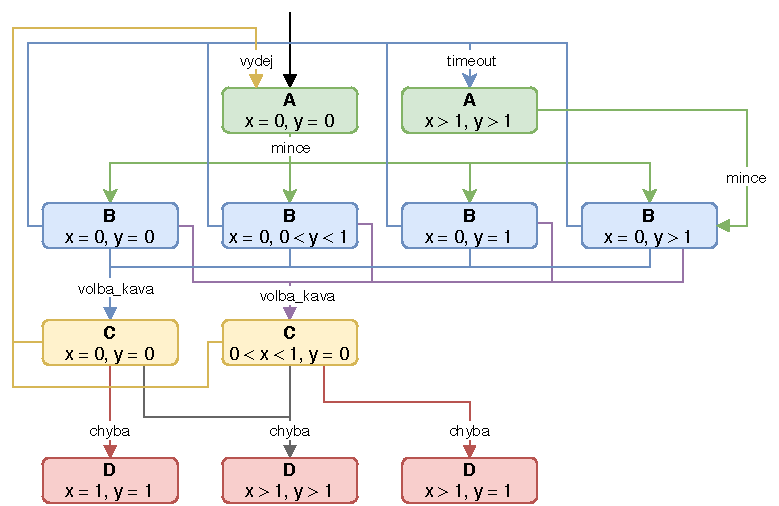
\includegraphics[width=.8 \linewidth]{img/region-abstraction.pdf}
    \end{center}

    \begin{itemize}
        \item
            \textbf{Stav, ve kterém platí predikát $ \boldsymbol{error} $, je
            dostupný.} Existuje běh $ (A; x = 0, y = 0) \xrightarrow{\mathtt{
            mince}} (B; x = 0, y = 0) \xrightarrow{\mathtt{volba\_kava}} (C;
            x = 0, y = 0) \xrightarrow{1, \mathtt{chyba}} (D; x = 1, y = 1) $,
            kde $ A \in Loc_0 \wedge error \in L(D) $. Dostupnost tohoto
            stavu s~tímto predikátem je také vidět v~regionové abstrakci.

        \item
            \textbf{Tvrzení $ \boldsymbol{\mathcal{A}_2 \models \exists\,(
            run\ U^{< 2}\ error)} $ platí}. Platí, že $ Int_{\mathcal{A}_2}
            \subseteq Sat(\phi) $, kde $ \phi \equiv \exists\,(run\ U^{< 2}
            \ error) $, $ Int_{\mathcal{A}_2} = \{s = (A; x = 0, y = 0)\} $
            a~$ s \models \phi $, protože existuje cesta $ \pi \in Path_{div}(
            s) $, pro kterou platí $ \pi \models run\ U^{< 2}\ error $.
            Cesta~$ \pi $ může být např. následující $ \pi = (A; x = 0, y = 0)
            \xrightarrow{\mathtt{ mince}} (B; x = 0, y = 0) \xrightarrow{
            \mathtt{volba\_kava}} (C; x = 0, y = 0) \xrightarrow{1, \mathtt{
            chyba}} (D; x = 1, y = 1) \xrightarrow{\tau} (D; x = 1 + \tau, y =
            1 + \tau) \xrightarrow{\tau} \dots $; $ \pi \models run\ U^{< 2}
            \ error $, protože existuje časový okamžik $ t = 1 $ z~intervalu
            $ [0, 2) $, ve kterém platí formule $ error $ ($ error \in L(D) $)
            a~pro libovolný časový okamžik menší než~$ t $~platí $ run \vee
            error $. Toto lze vypozorovat v~regionové abstrakci.

        \item
            \textbf{Tvrzení $ \boldsymbol{(B; x = 0, y = 0) \models \forall\,(
            run\ U^{< 2}\ init)} $ neplatí.} Neplatí totiž, že pro každou
            cestu $ \pi \in Path_{div}(s) $ platí $ \pi \models \phi $,
            kde $ s = (B; x = 0, y = 0) $ a~$ \phi \equiv run\ U^{< 2}\ init $.
            Např. pro cestu $ \pi = (B; x = 0, y = 0) \xrightarrow{10} (B; x =
            10, y = 10) \xrightarrow{\tau} (B; x = 10 + \tau, y = 10 + \tau)
            \xrightarrow{\tau} \dots $ neplatí $ \pi \models \phi $, protože
            zde neexistuje takový časový okamžik~$ t $ z~intervalu $ [0, 2) $,
            ve kterém by platila formule $ init $. Toto lze vypozorovat
            v~regionové abstrakci.
    \end{itemize}
\end{document}
